%% This is an example first chapter.  You should put chapter/appendix that you
%% write into a separate file, and add a line \include{yourfilename} to
%% main.tex, where `yourfilename.tex' is the name of the chapter/appendix file.
%% You can process specific files by typing their names in at the 
%% \files=
%% prompt when you run the file main.tex through LaTeX.
\chapter{Analysis Procedures}
In this chapter, the procedures of the search of excited leptons in $2e2\mu$ final state is described. The data and Monte-Carlo(MC) samples used in this analysis, search strtegies, and the final selected yields will be reported. Some information of $4\mu$ and $4e$ channel will be refered as well in order to provide a complete picture of this search, although this thesis mainly focuses on $2e2\mu$ channels.     

\section{Data and Monte-Carlo samples}
\label{sec:Samples}
\subsection{Data samples}
In this analysis, the full CMS data collected in 2012 is used, corresponding to the integrated luminosity of 19.7 $\pm$ 0.5 fb$^{-1}$\cite{lumi001}. The data were recorded at a centre-of-mass energy of $\sqrt{s}=8$ TeV and analyzed with the CMSSW53X software. There are 4 channels and 3 datasets used in this analysis. $\mu \mu^{*} \rightarrow 4\mu$ uses the double muon dataset. $\mu \mu^{*} \rightarrow 2\mu2e$, and $e e^{*} \rightarrow 2e2\mu$ relies on muon-photon dataset. $e e^{*} \rightarrow 4e$ rides on double electron dataset. The full dataset names are listed in Tab. \ref{tab:DatasetName}. The name of dataset reveals the information of the trigger selection, which will be described in next section.  

\begin{center}
\begin{table}[h!]
\begin{center}
\begin{tabular}{|l|l|}
\hline
CMS Run Range & Dataset Name \\
\hline
190456 - 193621 & /DoubleMu/Run2012A-22Jan2013-v1/AOD \\
& /DoubleElectron/Run2012A-22Jan2013-v1/AOD \\
& /MuEG/Run2012A-22Jan2013-v1/AOD \\
\hline
193833 - 196531 & /DoubleMuParked/Run2012B-22Jan2013-v1/AOD \\
& /DoubleElectron/Run2012B-22Jan2013-v1/AOD \\
& /MuEG/Run2012B-22Jan2013-v1/AOD \\
\hline
198022 - 203742 & /DoubleMuParked/Run2012C-22Jan2013-v1/AOD \\
& /DoubleElectron/Run2012C-22Jan2013-v1/AOD \\
& /MuEG/Run2012C-22Jan2013-v1/AOD \\
\hline
203777 - 208686 & /DoubleMuParked/Run2012D-22Jan2013-v1/AOD \\
& /DoubleElectron/Run2012D-22Jan2013-v1/AOD \\
& /MuEG/Run2012D-22Jan2013-v1/AOD \\
\hline

\end{tabular}
\end{center}
\caption{\label{tab:DatasetName}Summary of the data samples used in this analysis}
\end{table}
\end{center}

\subsection{Monte Carlo samples}

Tab. \ref{tab:signalsmustar} and \ref{tab:backgrounds} summarize the information on Monte Carlo(MC) samples used for signals and backgrounds. The MC samples were processed with different generators and ran through a GEANT4 \cite{Allison:2006ve} detector simulation. For the signals, leading order(LO) cross sections with a k-factor for QCD corrections \cite{kfactor} are used. Cross sections show in Tab. \ref{tab:signalsmustar} are calculated with $f = f^{\prime} = 1$. For $f = -f^{\prime} = -1$, where $\gamma$-mediated channel is forbidden, the cross sections are 3.5 times larger than $f = f^{\prime} = 1$ case. Background samples use next-to-leading order(NLO) cross sections. Both of signal and background MC samples are produced with the Summer12 MC conditions. For the background, samples are the one officially produced with PYTHIA, MADGRAPH \cite{madgraph} and POWHEG \cite{Alioli:2008gx} in CMS experiment. \newline
The signal samples are produced with PYTHIA 8 \cite{Sjostrand:2006za} at $\Lambda = 10$ TeV. {\sc Pythia8} can only simulate the production via contact interaction and the decay via gauge interaction. The calculation of the {\sc Pythia8} cross section is done via

\begin{align}
  \sigma_{ll^{*}\rightarrow llZ\rightarrow 2l2l'}^{Pythia\,8} = \frac{\Gamma_{Z}\cdot \Gamma_{Z\rightarrow ll}}{\Gamma_{Z} + \Gamma_{W} + \Gamma_{\gamma}} \cdot \sigma_{ll^{*}}^{Pythia\,8} = \frac{\Gamma_{Z}\cdot \Gamma_{Z\rightarrow ll}}{\Gamma_{G}} \cdot \sigma_{ll^{*}}^{Pythia\,8}
\end{align}

\noindent where $\Gamma_{G}$ is the decay width of all gauge interaction decays. However, it is possible that the excited lepton decays via contact interaction instead of gauge interaction. In this case, the cross section calculated by Pythia 8 will be overestimated. The actual cross section of excited lepton decay via Z boson should have form  

\begin{align}
  \sigma_{ll^{*}\rightarrow llZ\rightarrow 2l2l'} = \frac{\Gamma_{Z}\cdot \Gamma_{Z\rightarrow ll}}{\Gamma_{G} + \Gamma_{CI}} \cdot \sigma_{ll^{*}}
\end{align}

\noindent with the contact interaction decay width $\Gamma_{CI}$ included. To get this cross section, the one given by Pythia 8 has to be scaled with the correction factor

\begin{align}
  c = \frac{\Gamma_{G}}{\Gamma_{G} + \Gamma_{CI}}.
\end{align}

\noindent This factor strongly depends on the ratio $M_{l^{*}} / \Lambda$. This is due to the different dependance of $M_{l^{*}} / \Lambda$ in $\Gamma_{CI}$ and $\Gamma_{G}$. $\Gamma_{CI}$ is a function of $M_{l^{*}}^{5} / \Lambda^{4}$ while $\Gamma_{G}$ is a function of $M_{l^{*}}^{3} / \Lambda^{2}$. This indicates that the contact interaction will be dominate as $M_{l^{*}}$ apporaches $\Lambda$. For example, for $\Lambda = 10$ TeV and $M_{l^{*}} =$ 200 GeV, the factor c = 0.993 while for a mass of 2600 GeV, it decreases to c = 0.538. The lowest value of this factor is given at $M_{l^{*}} = \Lambda$ with c = 0.07. The importance of scaling down the cross section calculated by Pythia 8 is to give out a more conservative result of the search, avoiding an overestimated upper limit. 


\begin{table}[h!]
\begin{center}
\begin{tabular}{|l|c|c|c|c|}
\hline
$M_{l^{*}}$ & cross section $\times$ BR & cross section $\times$  & \multirow{2}{*}{k-factor} & \multirow{2}{*}{\# events $\mu^{*} / e^{*}$} \\
(GeV) & without CI decay (pb) & incl. CI decay (pb) &  &  \\
\hline
200 & $2.095\cdot 10^{-4}$ & $2.081\cdot 10^{-4}$ & 1.296 & 8500 / 8500\\
400 & $1.363\cdot 10^{-4}$ & $1.334\cdot 10^{-4}$ & 1.290 & 10000 / 10000\\
600 & $8.122\cdot 10^{-5}$ & $7.757\cdot 10^{-5}$ & 1.282 & 10000 / 8000\\
800 & $4.817\cdot 10^{-5}$ & $4.449\cdot 10^{-5}$ & 1.273 & 9000 / 10000\\
1000 & $2.844\cdot 10^{-5}$ & $2.520\cdot 10^{-5}$ & 1.268 & 10000 / 10000\\
1200 & $1.675\cdot 10^{-5}$ & $1.414\cdot 10^{-5}$ & 1.265 & 8000 / 10000\\
1400 & $9.786\cdot 10^{-6}$ & $7.826\cdot 10^{-6}$ & 1.267 & 9000 / 10000\\
1600 & $5.686\cdot 10^{-6}$ & $4.286\cdot 10^{-6}$ & 1.272 & 10000 / 10000\\
1800 & $3.286\cdot 10^{-6}$ & $2.325\cdot 10^{-6}$ & 1.282 & 10000 / 10000\\
2000 & $1.875\cdot 10^{-6}$ & $1.242\cdot 10^{-6}$ & 1.295 & 10000 / 10000\\
2200 & $1.062\cdot 10^{-6}$ & $6.569\cdot 10^{-7}$ & 1.311 & 10000 / 10000\\
2400 & $5.936\cdot 10^{-7}$ & $3.424\cdot 10^{-7}$ & 1.329 & 10000 / 10000\\
2600 & $3.280\cdot 10^{-7}$ & $1.763\cdot 10^{-7}$ & 1.348(*) & 10000 / 10000\\
\hline

\end{tabular}
\end{center}
\caption{\label{tab:signalsmustar}Summary of Monte Carlo signal samples, cross sections (LO), and k-factors used for $ll^{*} \rightarrow ll Z \rightarrow 2l 2l'$ ($l = e,\mu$ and $l' = e,\mu,\tau$) with $\Lambda$ = 10 TeV and $f = f^{\prime} = 1$. (*) The k-factor for 2600 GeV was calculated by extrapolation \cite{kfactor}. }
\end{table}


\begin{center}
\begin{sidewaystable}[h]
\begin{center}
\begin{tabular}{|l|l|c|}
\hline
Process & Dataset Name & Cross section (pb) \\
\hline
$q \bar{q} \rightarrow ZZ \rightarrow 4e$ & $/ZZTo4e\_8TeV-powheg-pythia6$ & 0.07691 \\
$q \bar{q} \rightarrow ZZ \rightarrow 4\mu$ & $/ZZTo4mu\_8TeV-powheg-pythia6$ & 0.07691 \\
$q \bar{q} \rightarrow ZZ \rightarrow 4\tau$ & $/ZZTo4tau\_8TeV-powheg-pythia6$ & 0.07691 \\
$q \bar{q} \rightarrow ZZ \rightarrow 2e2\mu$ & $/ZZTo2e2mu\_8TeV-powheg-pythia6$ & 0.1767 \\
$q \bar{q} \rightarrow ZZ \rightarrow 2e2\tau$ & $/ZZTo2e2tau\_8TeV-powheg-pythia6$ & 0.1767 \\
$q \bar{q} \rightarrow ZZ \rightarrow 2\mu 2\tau$ & $/ZZTo2mu2tau\_8TeV-powheg-pythia6$ & 0.1767 \\
$gg \rightarrow ZZ \rightarrow 2l 2l'$ & $/GluGluToZZTo2L2L\_8TeV-gg2zz-pythia6$ & 0.01203 \\
$gg \rightarrow ZZ \rightarrow 4l$ & $/GluGluToZZTo4L\_8TeV-gg2zz-pythia6$ & 0.0048 \\
$WZ \rightarrow 3l\nu$ & $/WZJetsTo3LNu\_TuneZ2\_8TeV-madgraph-tauola$ & 1.057 \\
$WZ \rightarrow 2l2q$ & $/WZJetsTo2L2Q\_TuneZ2star\_8TeV-madgraph-tauola$ & 1.755 \\
$ttZ$ & $/TTZJets\_8TeV-madgraph\_v2$ & 0.208 \\
$ttW$ & $/TTWJets\_8TeV-madgraph$ & 0.232 \\
$tt\gamma$ & $/TTGJets\_8TeV-madgraph$ & 2.17 \\
$ttWW$ & $/TTWWJets\_8TeV-madgraph$ & 0.002 \\
$WWG$ & $/WWGJets\_8TeV-madgraph$ & 1.44 \\
$WWZ$ & $/WWZNoGstarJets\_8TeV-madgraph$ & 0.0633 \\
$WZZ$ & $/WZZNoGstarJets\_8TeV-madgraph$ & 0.0197 \\
$ZZZ$ & $/ZZZNoGstarJets\_8TeV-madgraph$ & 0.0046 \\
\hline

\end{tabular}
\end{center}
\caption{\label{tab:backgrounds} Summary of the used Monte Carlo background samples with the corresponding cross section in NLO.}
\end{sidewaystable}
\end{center}

\pagebreak
\newpage

\section{Trigger}

\label{sec:trigger}Three different triggers are used in this search. $\mu\mu^{*} \rightarrow \mu\mu Z \rightarrow 4\mu$ channel uses the double muon trigger with at least one 17 GeV muon and one 8 GeV muon, $HLT\_Mu17\_Mu8\_v*$. For $e e^{*} \rightarrow e e Z \rightarrow 4e$, the double elctron trigger with at least one 17 GeV electron and one 8 GeV electron, $HLT\_Ele17\_Ele8\_v*$, is used. The two cross channels $\mu\mu^{*} \rightarrow \mu\mu Z \rightarrow 2\mu 2e$ and $e e^{*} \rightarrow e e Z \rightarrow 2e 2\mu$ use the muon-photon trigger with at least one muon and one photon excess 22 GeV, $HLT\_Mu22\_Photon22\_*$.
\newline
The choice of the trigger in $4\mu$ and $4e$ are pretty intuitive, but why is the muon-photon trigger used in the $2e2\mu$ channels? The reason is the muon-electron trigger is inefficient in the $\mu\mu^{*} \rightarrow \mu\mu Z \rightarrow 2\mu 2e$ channel due to the isolation requirement for electrons in trigger. In high mass signal regions, Z boson from $\mu^{*}$ decay may be highly boosted, it causes the electron pair decaying from boosted Z too close to each other, and furthermore is rejected by the isolation requirement of electron in trigger. Fortunately, an electron acts similarily to a photon in the electromegnetic calorimeter, every electron is also a photon in this stage of analysis. This characteristic offers a great oppurtunity to use muon-photon trigger, which does not include isolation requirements on photon, instead of muon-electron trigger to avoid the issue of isolation requirement. The performance of different triggers as a function of excited lepton mass for both $2e2\mu$ channels are shown in Fig. \ref{fig:TrgEff}. Though the muon-electron trigger is only inefficient in $\mu\mu^{*} \rightarrow 2\mu2e$, for convience, both channels are analyzed with the same muon-photon trigger. The muon-photon trigger efficiencies are close to one in both cases.

\begin{figure}[hp!]
\begin{center}
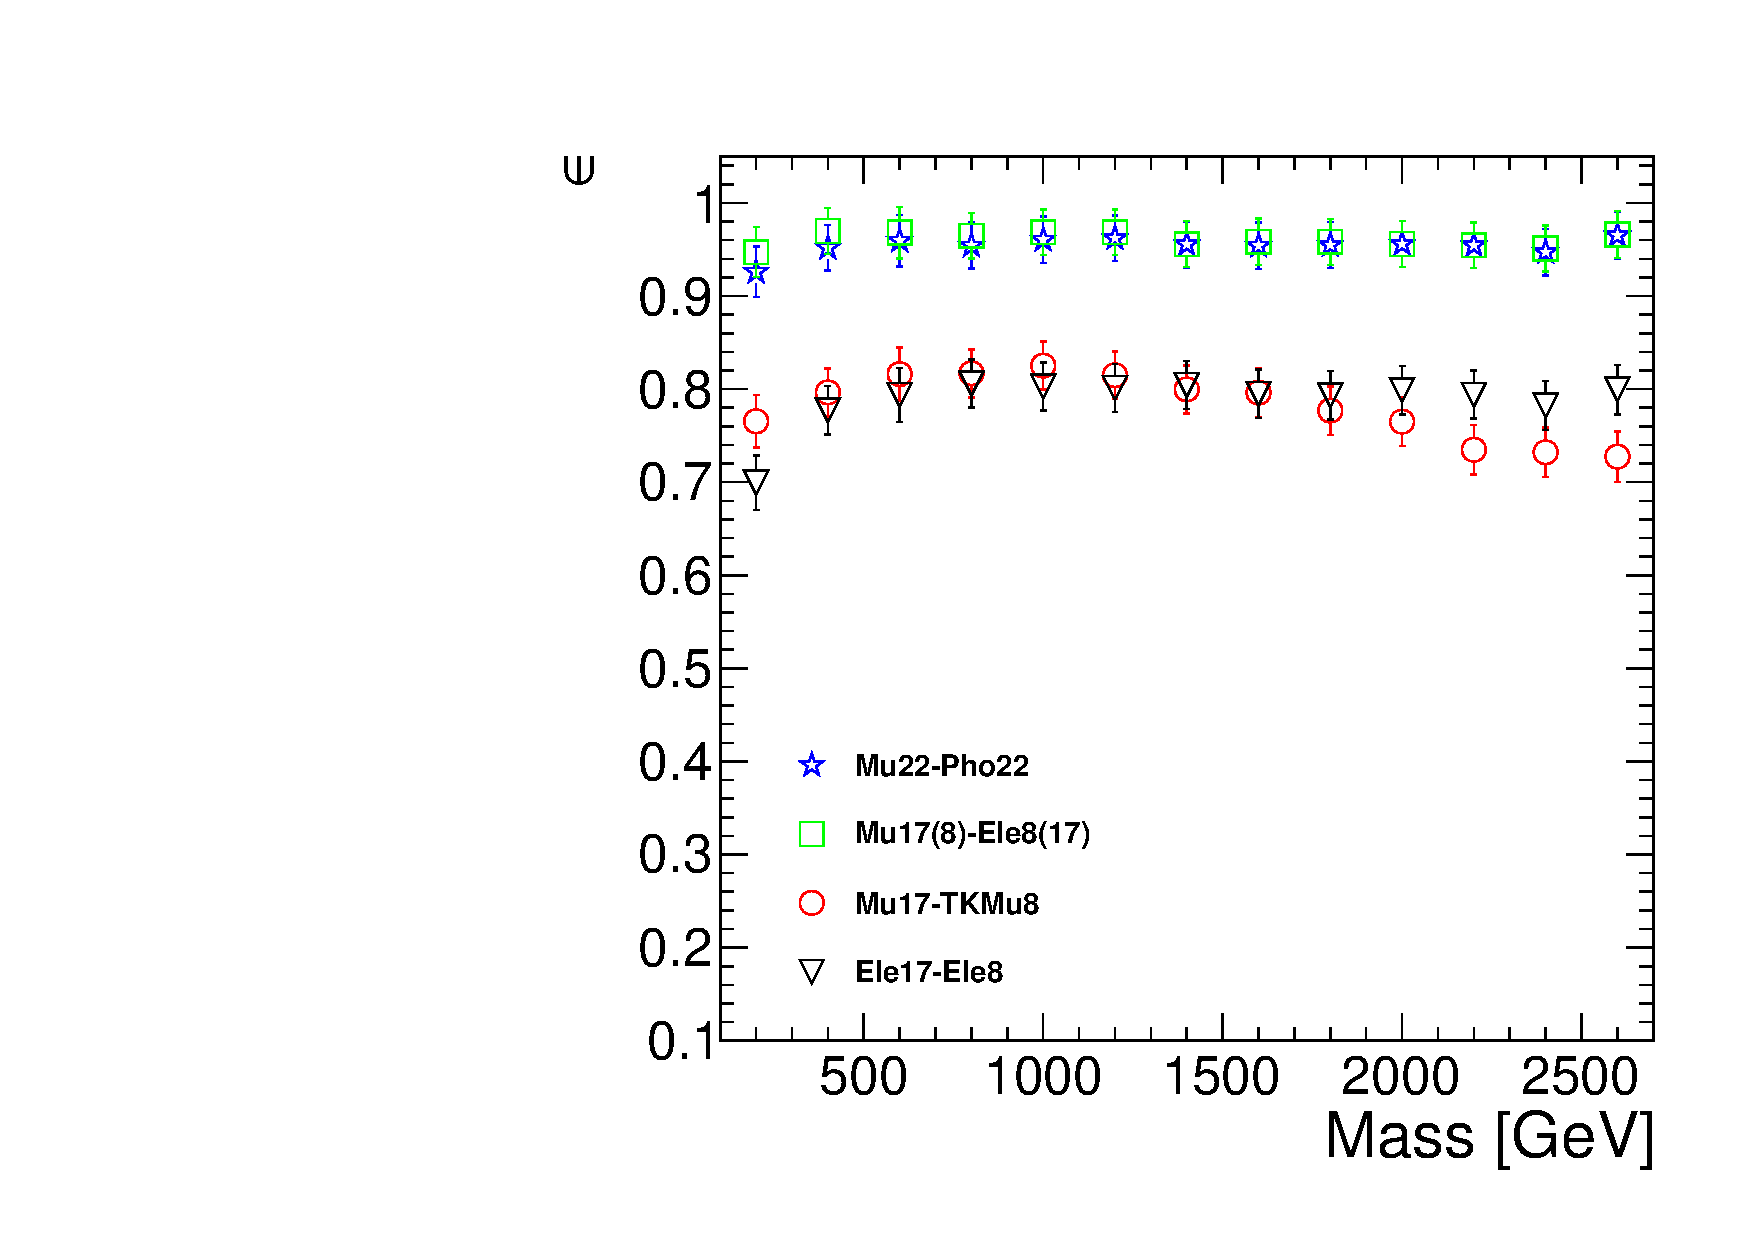
\includegraphics[width=0.7\textwidth]{plot/TrgEff_estar.pdf}
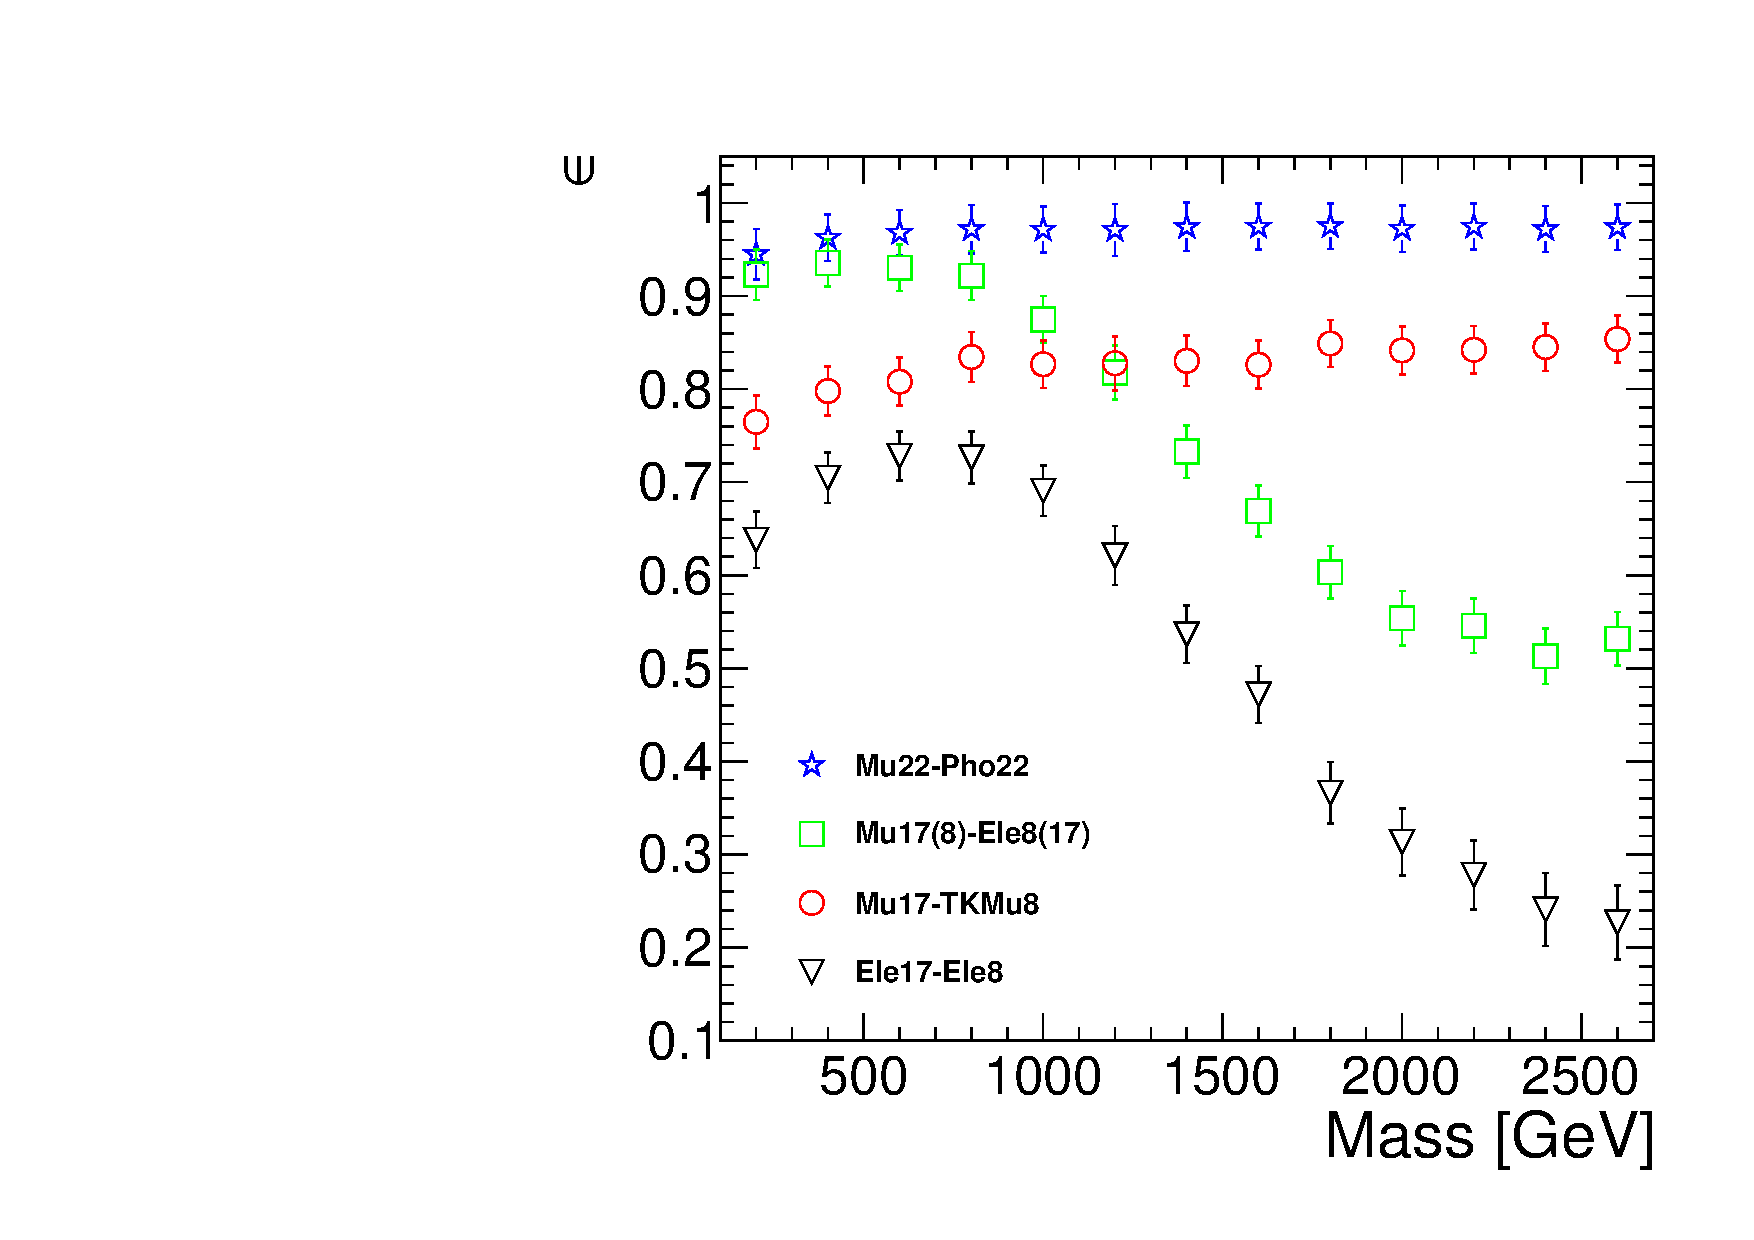
\includegraphics[width=0.7\textwidth]{plot/TrgEff_mustar.pdf} \\
\end{center}
\caption{\label{fig:TrgEff}The comparison of different trigger efficiencies as a function of excited lepton mass for both $2e2\mu$ channels. Top: $ee^{*}\rightarrow2e2\mu$ channel. Bottom: $\mu\mu^{*}\rightarrow2\mu2e$ channel.}
\end{figure}

\section{Object reconstruction and identification}

\subsection{Electron reconstruction}
Electron is a particle that involves in various electroweak decays in the experiment. An electron in the CMS experiment leaves the footprint in tracker and deposite its entire energy in ECAL. Therefore, to reconstruct an electron, it's essential to find a brilliant way to match the information acquired in both of tracker and ECAL.   
\subsection*{ECAL clustering}
For electrons, which deposite their entire energy to several crystals in ECAL, clustering is an important step for energy reconstruction. For every single hit in ECAL from an electron or a photon, approximately 94\% of energy is contained in $3\times3$ crystals, and 97\% in $5\times5$ crystals. To form a basic cluster, crystals with $E_{T} > 1 GeV$ are picked up as seeds. Then, starting from seed crystal, dominos of size 1 $\times$ 3 or  1 $\times$ 5 are created in $\eta -\phi$ plane. Energy of these dominos are then added up along $\phi$ direction if energy of a domino exceed 0.1 GeV threshold.     
  However, a single energy cluster can not reconstruct the energy well enough for an electron or a photon in real world, which involves bremsstrahlung and conversion process.\newline
During the flight through the detectors under strong magnetic field, each electron may create several photons due to bremsstrahlung along $\phi$ directrion. To correctly reconstruct the energy of an electron, it is needed to take the energy of photons from bremsstrahlung into account to form a larger cluster, called supercluster. The concept of superclustering is to collect the energy along the $\phi$ direction starting from the position of the seed crystal with a fixed $\eta$ width. The technical details of the clustering can be found in \cite{ptdr1}.
\subsection*{Electron tracking}
The track reconstruction in CMS experiment contains several steps. First, the hit on the pixel and the tracker should be reconstructed. The second step is to find the seed of tracks by matching at least 2 hits in pixel detector. The last step is to fit the trajectory starting from the seed\cite{GSF,ptdr1}. In general case, Kalman filter(KF) is used to fit the trajectory\cite{trkreco}, but it is not suitable for electrons due to the relatively large energy loss in bremsstrahlung. Therefore, the Gaussian-sum filter(GSF) algorithm is developed to substitute the KF for electron reconstruction\cite{GSF}. In GSF algorithm, the energy loss probability density function is constructed by multiple Gaussians instead of a single Gaussian as described in Bethe-Heitler model\cite{BHmodel}. It turns out that GSF provide a better momentum resolution than KF, and the GSF algorithm is used in electron reconstruction\cite{GSF}. Finally, the electrons are built by matching the supercluster to the GSF track. The reconstruction efficiency of electrons $E_{T}$ greater than 20 GeV is generally above 95\%(90\%) in EB(EE)\cite{eRecoEff}.

\subsection{Electron identification}
\label{sec:ElectronID}The high $p_{T}$ electron selection used in this analysis (HEEP selection \cite{heepeid}) starts from a GSF electron on which kinematic, identification(ID) and isolation(Iso) cuts are applied. The major difference between HEEP selection and standard electron selection is the use of electron energy measurement. Later one is measured by the combination of tracker and Ecal information. However, under certain situations, one can discard the calorimeter energy completely (most likely in the crack region) and just use the track momentum, while calorimeter measurement is highly dominated in high $p_{T}$ region. In this case, if the track is badly reconstructed, it might cause a low $p_{T}$ electron to become a high $p_{T}$ one. To avoid this problem, HEEP selection always takes energy of the supercluster as the energy of an electron. The requirements used in electron selection are as follows.
\begin{itemize}
\item Kinematic requirements: Electrons with $E_{T}$ $>$ 25 GeV and $|\eta_{SC}|$ $<$ 2.5 but not within the transition region between EB and EE
\item Is ECAL driven: Electrons should be reconstructed from an ECAL seed
\item $\Delta\eta_{in}$: The difference in $\eta$ between the track position measured in the inner tracker layers and the $\eta$ of the supercluster
\item $\Delta\phi_{in}$: The difference in $\phi$ between the track position measured in the inner tracker layers and the $\phi$ of the supercluster
\item H/E: The ratio of the hadronic energy in a cone of radius 0.15 centred on the electron's position in the calorimeter to the electromagnetic energy of the electron's supercluster
\item $\sigma_{i\eta i\eta}$: A measure of the spread in eta in units of crystals of the electrons energy in the 5x5 block centred on the seed crystal
\item $E_{2\times5}/E_{5\times5}$: The maximum energy fraction of $2\times5$ crystal blocks(including seed crystal) in the $5\times5$ seed cluster 
\item $E_{1\times5}/E_{5\times5}$: The maximum energy fraction of $1\times5$ crystal blocks(including seed crystal) in the $5\times5$ seed cluster 
\item Inner layer lost hits: Number of lost hits in inner tracker
\item $d_{xy}$: The distance between the electron track and the primary vertex in x-y plane
\item $Iso_{Trk}$: The sum of tracks' $p_{T}$ in a $\Delta R$ cone of 0.04 to 0.3 centered at electron position  
\item $Iso_{Ecal}$: The sum of $E_{T}$ in a $\Delta R$ cone of 0.3 centered at electron position, excluding the inner cone of 3 crystals in Ecal
\item $Iso_{Hcal}$: The sum of $E_{T}$ in a $\Delta R$ cone of 0.15-0.3 centered at electron position in Hcal 
\end{itemize}
The detail criteria of the selection are listed in Tab. \ref{tab:HeepEid}. When the electrons decay from a highly boosted Z boson, they might get too closed to each other and fail the isolation requirement. Hence, the isolation is modified when $\Delta$R between two electrons is less than 0.3 by subtracting the contribution from the other electron. This modification is the same as what is done in boosted Z analysis \cite{ModEleIso}. The data and MC match each other well for used ID and isolation.To make MC simulation more likely to realistic, a ``scale factor'' is applied to MC samples to correct the selection efficiency difference between data and MC. For electron scale factor, the official numbers calculated by HEEP group in CMS is applied\cite{heepSFsyst} as shown in Tab. \ref{tab:SF_heep}.    

\begin{table}[hp]
\begin{center}
\begin{tabular}{|l|c|c|}
\hline
Variable & Barrel & Endcap \\
\hline
$E_{T}$ & $>$ 25 GeV & $>$ 25 GeV \\
$|\eta_{SC}|$ & $|\eta_{SC}|$ $<$ 1.442 & 1.56 $<$ $|\eta_{SC}|$ $<$ 2.5 \\
Is Ecal Driven & yes & yes \\
$|\Delta\eta_{in}|$ & $<$ 0.005 & $<$ 0.007 \\
$|\Delta\phi_{in}|$ & $<$ 0.06 & $<$ 0.06 \\
H/E & $<$ 0.05 & $<$ 0.05 \\
$\sigma_{i\eta i\eta}$ & - & $<$ 0.03 \\
$E^{2\times5}/E^{5\times5}$ & $>$ 0.94 & - \\
 & or $E^{1\times5}/E^{5\times5}$ $>$ 0.83 & \\
Inner Layer Lost Hits & $<=$ 1 & $<=$ 1 \\
$|d_{xy}|$ & $<$ 0.02 cm & $<$ 0.05 cm\\
\hline
$Iso_{Ecal+Hcal}$  & $<$ 2 + 0.03$E_{T}$ + 0.28$\rho$ GeV & $<$ 2.5 + 0.28$\rho$ GeV for $E_{T} <$ 50 GeV \\
 & & $<$ 2.5 + 0.03($E_{T}$-50) + 0.28$\rho$ GeV others \\
$Iso_{Trk}$  & $<$ 5 GeV& $<$ 5 GeV\\
\hline
\end{tabular}
\caption{HEEP electron ID}
\label{tab:HeepEid}
\end{center}
\end{table}

\begin{table}[hp]
\begin{center}
\begin{tabular}{|l|c|c|}
\hline
 & E$_{T} <$ 100 GeV & E$_{T} >$ 100 GeV \\
\hline
0 $< |\eta| <$ 1.4442 & 0.997 $\pm$ 0.000 & 0.985 $\pm$ 0.002 \\
1.4442 $< |\eta| <$ 1.566 & 0.979 $\pm$ 0.000 & 0.981 $\pm$ 0.006 \\
\hline
\end{tabular}
\caption{\label{tab:SF_heep}Scale factors for HEEP electron selection from HEEP group}
\end{center}
\end{table}

\subsection{Muon reconstruction}
Muon is an important object in CMS experiment. Even the name of the experiment contains the word ``muon''. It is a kind of lepton just as electron and almost every electron-related process have also a muon-related channel. Muon leaves it's footprints in tracker like electron, but it only deposits little of its energy in calorimeter. Nothing in CMS can stop muon's flight as long as it isn't super soft. It is the only kind of particle that can reach the outermost muon chamber and escape the detector to the outside world. This characteristic makes muon a highly recognized object in the experiment. The reconstruction efficiency is about 99\% for the muon carries enough high momentum within detector coverage\cite{mureco}.\newline
The reconstruction of muon track is first done independently by tracker(tracker track) and muon chamber(standalone track). There are two main approaches to match the track in tracker and muon chamber and bring out two different types of muon.
\begin{itemize}
\item Global muon: Starting from the reconstructed standalone track, the global muon algorithm finds a best tracker track to match the standalone track. Then, the global muon track is fitted by combining hits from the standalone track and tracker track using KF technique\cite{trkreco}. For high $p_{T}$ muons up to 200 GeV, the global fit can improve the momentum resolution compared to the tracker-only fit\cite{mureco}.
\item Tracker muon: A tracker muon is reconstructed by an opposite direction from a global muon. The tracker muon algorithm starts from the tracker track, and finds if there is at least one muon segment(muon segment is the short track form by the hits in DT or CSC. It's not a stanalone track, which needs to match a muon ``hits'' in RPC) to match to the extrapolated track. It's  more efficient than global fit for muon with only serveral GeV momentum, but for the muon used mostly in physics analysis, a muon is often reconstructed as a global muon and tracker muon simutaneously\cite{mureco}.   
\end{itemize}   

\subsection{Muon identification}

\label{sec:MuonID}To select the muon, the "High p$_{T}$ ID" from the muon POG is used \cite{ExoMu}. The requirements used in muon selection are listed as follows:  

\begin{itemize}
	\item Kinematic requirements: Muons should have $p_{T}$ $>$ 25 GeV and $|\eta|$ $<$ 2.4
	\item Muon is a global muon
	\item Number of muon hits in the global track 
	\item Muon stations: Number of muon segments in muon chamber  
	\item $d_{xy}$: The distence between the muon track and the primary vertex in x-y plane
	\item $d_{z}$: The distence between the muon track and the primary vertex in z direction
	\item Number of pixel hits 
	\item Number of tracker layers with hits 
	\item $\Delta p_{T}/p_{T}$: The ratio of the transverse momentum error to it's transverse momentum      
	\item $Iso_{TrkRel}$: The relative isolation computed by the ratio of tracks $p_{T}$ in a cone of $\Delta R$ 0.04-0.3 centered at muon tracks to muon's $p_{T}$    
\end{itemize}

For the second muon of the Z decay(in $ee^{*} \rightarrow 2e2\mu$ channel), the ID is slightly modified due to an inefficiency in the global muon reconstruction for boosted objects decaying into two muons because they are close to each other. While one of the two muons is reconstructed as a global muon, the other one is only reconstructed as a tracker muon. This task leads to an inefficiency for the signal if we apply the high-$p_{T}$ muon ID. To get around with this problem, the second muon is allowed to be a tracker muon instead of a global muon. Additionally, the requirement on the muon hits in the global tag is removed. The isolation of the two muons from the Z decay is also changed by removing the contribution of the other muon. Following statements are the modification to the high $p_{T}$ muon ID for the muons coming from boosted Z decay. 

\begin{itemize}
 	\item Muon doesn't have to be a global muon, but has to be a tracker muon
	\item Remove requirement for muon hits in global track
	\item Remove the contribution in $Iso_{TrkRel}$ calculation of the other muon when two muons' tracks are within $\Delta R <$ 0.3 
\end{itemize}
The Tab. \ref{tab:muid} summarized the muon selection criteria in this analysis.


\begin{table}[hp]
\begin{center}
\begin{tabular}{|l|c|c|}
\hline
Variable & Standard & Modified \\
\hline
$p_{T}$ & $>$ 25 GeV & $>$ 25 GeV \\
$|\eta|$ & $|\eta|$ $<$ 2.4 &  $|\eta|$ $<$ 2.4 \\
Muon type & Global muon & Tracker muon \\
Muon hits in global track & $>=$ 1 & - \\
Muon stations & $>=$ 2 & $>=$ 2 \\
$d_{xy}$ & $<$ 0.2 cm & $<$ 0.2 cm\\
$d_{z}$ & $<$ 0.5 cm & $<$ 0.5 cm\\
Pixel hits & $>=$ 1 & $>=$ 1 \\
Tracker layers & $>=$ 6 & $>=$ 6 \\
$\Delta p_{T}/p_{T}$ & $<$ 0.3 & $<$ 0.3 \\
\hline
$Iso_{TrkRel}$  & $<$ 0.1 & $<$ 0.1 \\
\hline
\end{tabular}
\caption{High $p{T}$ muon ID}
\label{tab:muid}
\end{center}
\end{table}


Fig. \ref{fig:Iso_Eff} shows the isolation efficiency of the different lepton pairs for muons and for electrons. To account for the differences between the MC and data efficiencies, the scale factors for the ID and isolation criteria are applied \cite{muoneff, muonresol, muoniso, muonTP}. The official numbers from the muon POG as shown in Tab.\ref{tab:SF_hptMu}-\ref{tab:SF_IsoTrkMu} are applied on the muons pass the un-modified muon ID and isolation. For the muons that pass the modified selection criteria, the numbers calculated from the $X \rightarrow ZZ \rightarrow 2q2l$ group \cite{XToZZTollqq} in Tab. \ref{tab:SF_ModMu} are applied because they used the same modifications as this analysis. The errors in the tables are statistical uncertainties, systematic uncertainties will be discussed in Sec. \ref{sec:Systematics}. The two cases to use the modified scale factors are:

\begin{enumerate}
	\item Muon passes the standard(global) high-$p_{T}$ ID leg with the modified isolation
	\item Muon passed the modified(tracker) high-$p_{T}$ ID leg with the modified isolation
\end{enumerate}

\begin{table}[hp]
\begin{center}
\begin{tabular}{|l|c|c|}
\hline
 & p$_{T} >$ 20 GeV & p$_{T} >$ 45 GeV \\
\hline
0 $< |\eta| <$ 0.9 & 0.9930 $\pm$ 0.0002 & 0.9900 $\pm$ 0.0003 \\
0.9 $< |\eta| <$ 1.2 & 0.9942 $\pm$ 0.0003 & 0.9923 $\pm$ 0.0006 \\
1.2 $< |\eta| <$ 2.1 & 0.9968 $\pm$ 0.0002 & 0.9949 $\pm$ 0.0004 \\
2.1 $< |\eta| <$ 2.4 & 0.9963 $\pm$ 0.0006 & 0.9923 $\pm$ 0.0012 \\
\hline
\end{tabular}
\caption{\label{tab:SF_hptMu}Scale factors for high-p$_{T}$ muon ID from MUO-POG}
\end{center}
\end{table}

\begin{table}[hp]
\begin{center}
\begin{tabular}{|l|c|c|}
\hline
 & p$_{T} >$ 20 GeV & p$_{T} >$ 45 GeV \\
\hline
0 $< |\eta| <$ 0.9 & 1.0001 $\pm$ 0.0001 & 0.9996 $\pm$ 0.0001 \\
0.9 $< |\eta| <$ 1.2 & 1.0006 $\pm$ 0.0001 & 0.9994 $\pm$ 0.0001 \\
1.2 $< |\eta| <$ 2.1 & 1.0006 $\pm$ 0.0001 & 0.9997 $\pm$ 0.0001 \\
2.1 $< |\eta| <$ 2.4 & 1.0005 $\pm$ 0.0001 & 0.9997 $\pm$ 0.0001 \\
\hline
\end{tabular}
\caption{\label{tab:SF_IsoTrkMu}Scale factors for TkRelIso $<$ 0.1 from MUO-POG}
\end{center}
\end{table}


\begin{table}[h!]
\begin{center}
    \begin{tabular}{|c|c|c|c|}
    \hline
    $|\eta|$ bin & $p_{T}$ (GeV) & GlobalID*ISO & TrackerID*ISO \\
    \hline
    \multirow{5}{*}{0 $< |\eta| <$ 0.9} & 20-40 & 0.9972 $\pm$ 0.0004 & 0.9989 $\pm$ 0.0004 \\
    & 40-60 & 0.9948 $\pm$ 0.0003 & 0.9973 $\pm$ 0.0003 \\
    & 60-80 & 1.0018 $\pm$ 0.0011 & 1.0029 $\pm$ 0.0010 \\
    & 80-100 & 1.0076 $\pm$ 0.0025 & 1.0096 $\pm$ 0.0023 \\
    & 100-500 & 1.0068 $\pm$ 0.0039 & 1.0075 $\pm$ 0.0037 \\
    \hline
    \multirow{5}{*}{0.9 $< |\eta| <$ 1.2} & 20-40 & 0.9971 $\pm$ 0.0007 & 0.9988 $\pm$ 0.0007 \\
    & 40-60 & 0.9963 $\pm$ 0.0005 & 0.9985 $\pm$ 0.0005 \\
    & 60-80 & 1.0014 $\pm$ 0.0022 & 1.0028 $\pm$ 0.0021 \\
    & 80-100 & 1.0060 $\pm$ 0.0049 & 1.0060 $\pm$ 0.0047 \\
    & 100-500 & 1.0058 $\pm$ 0.0080 & 1.0050 $\pm$ 0.0077 \\
    \hline
    \multirow{5}{*}{1.2 $< |\eta| <$ 2.1} & 20-40 & 1.0001 $\pm$ 0.0004 & 0.9999 $\pm$ 0.0005 \\
    & 40-60 & 0.9982 $\pm$ 0.0004 & 0.9985 $\pm$ 0.0004 \\
    & 60-80 & 1.0039 $\pm$ 0.0017 & 1.0039 $\pm$ 0.0016 \\
    & 80-100 & 1.0129 $\pm$ 0.0039 & 1.0081 $\pm$ 0.0036 \\
    & 100-500 & 1.0185 $\pm$ 0.0065 & 1.0180 $\pm$ 0.0063 \\
    \hline
    \multirow{5}{*}{2.1 $< |\eta| <$ 2.4} & 20-40 & 1.0015 $\pm$ 0.0030 & 1.0028 $\pm$ 0.0009 \\
    & 40-60 & 0.9955 $\pm$ 0.0012 & 0.9985 $\pm$ 0.0009 \\
    & 60-80 & 0.9929 $\pm$ 0.0071 & 0.9927 $\pm$ 0.0024 \\
    & 80-100 & 0.9834 $\pm$ 0.0092 & 0.9839 $\pm$ 0.0082 \\
    & 100-500 & 1.0438 $\pm$ 0.0160 & 1.0083 $\pm$ 0.0099 \\
    \hline
    \end{tabular}
\end{center}
\caption{\label{tab:SF_ModMu}Scale factors used for the modified muon ID and isolation, taken from $X \rightarrow ZZ \rightarrow qqll$ Analysis Note.}
\end{table}

\begin{figure}[hp]
\begin{center}
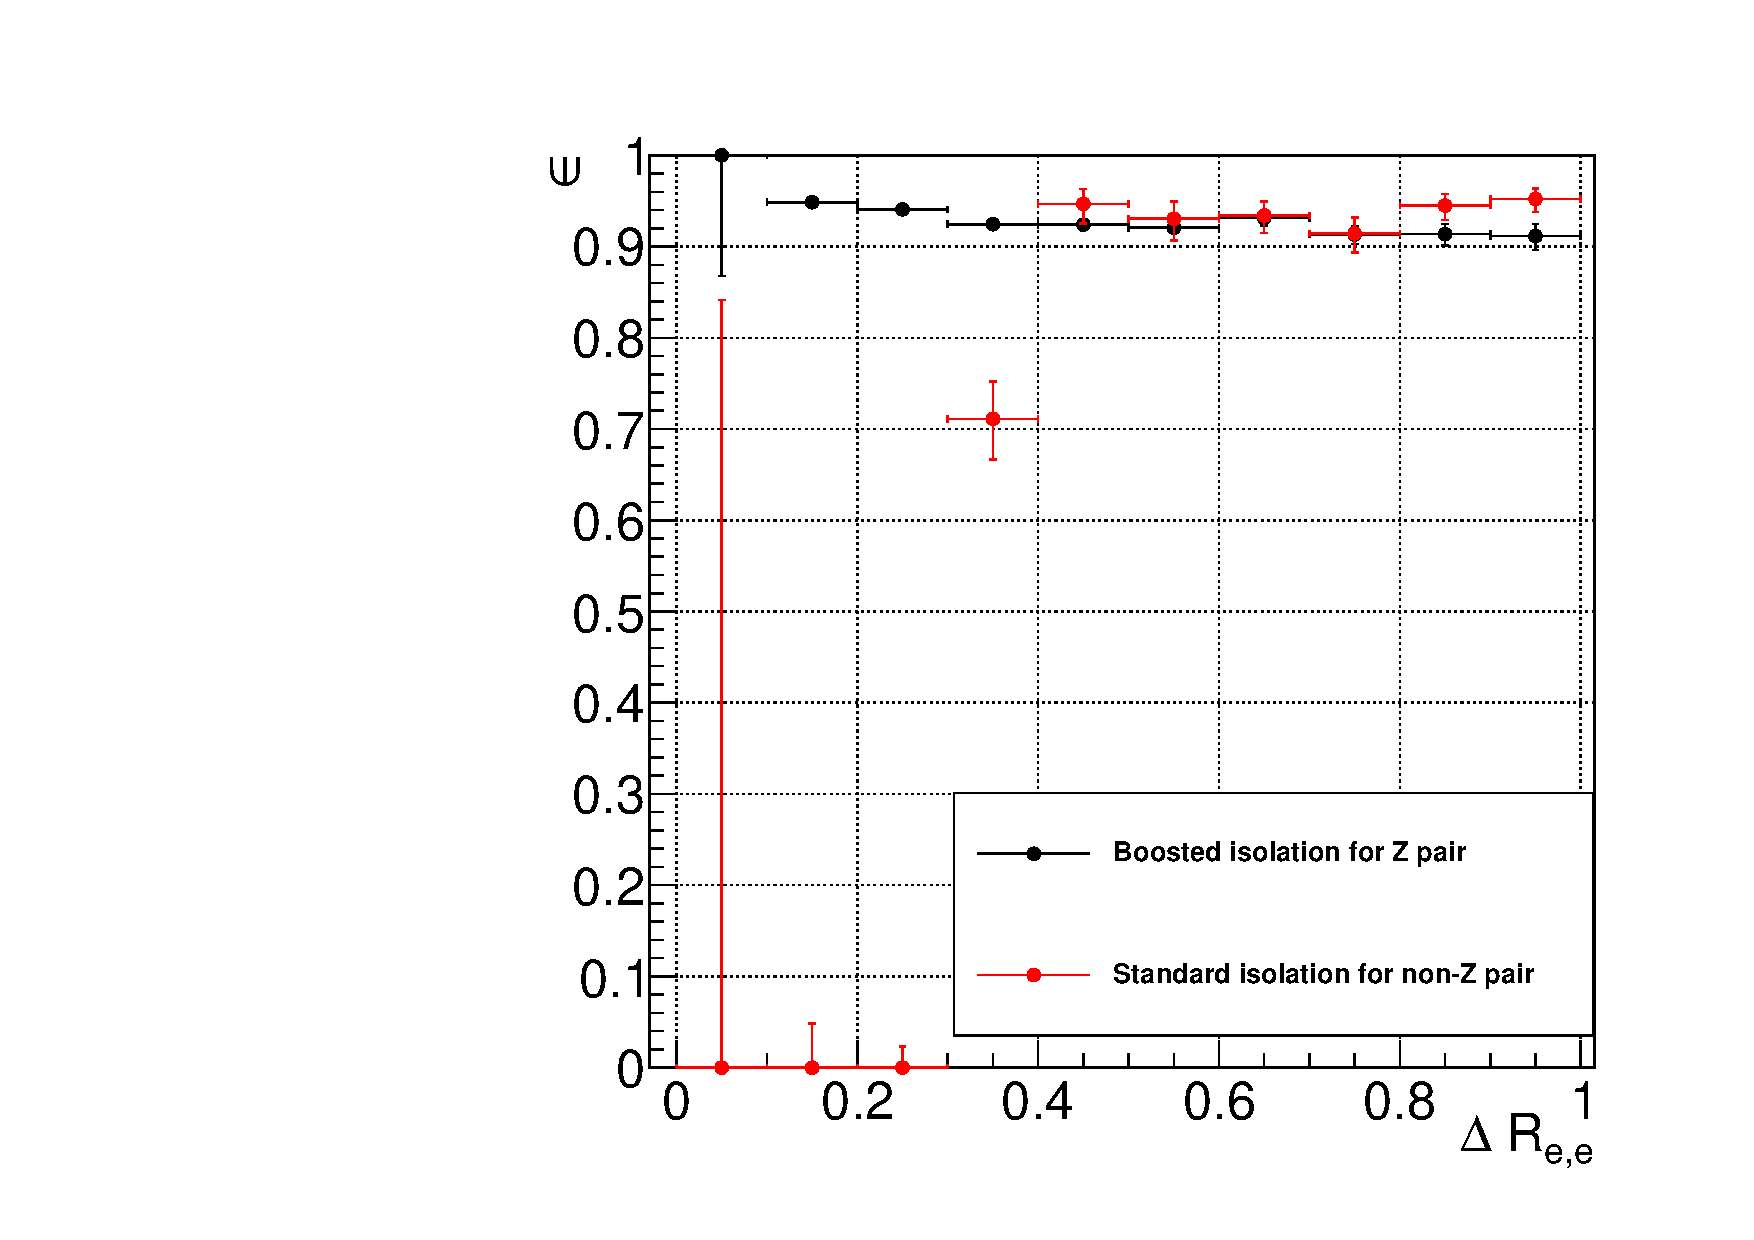
\includegraphics[width=0.5\textwidth]{plot/Isolation_electrons.pdf}\\
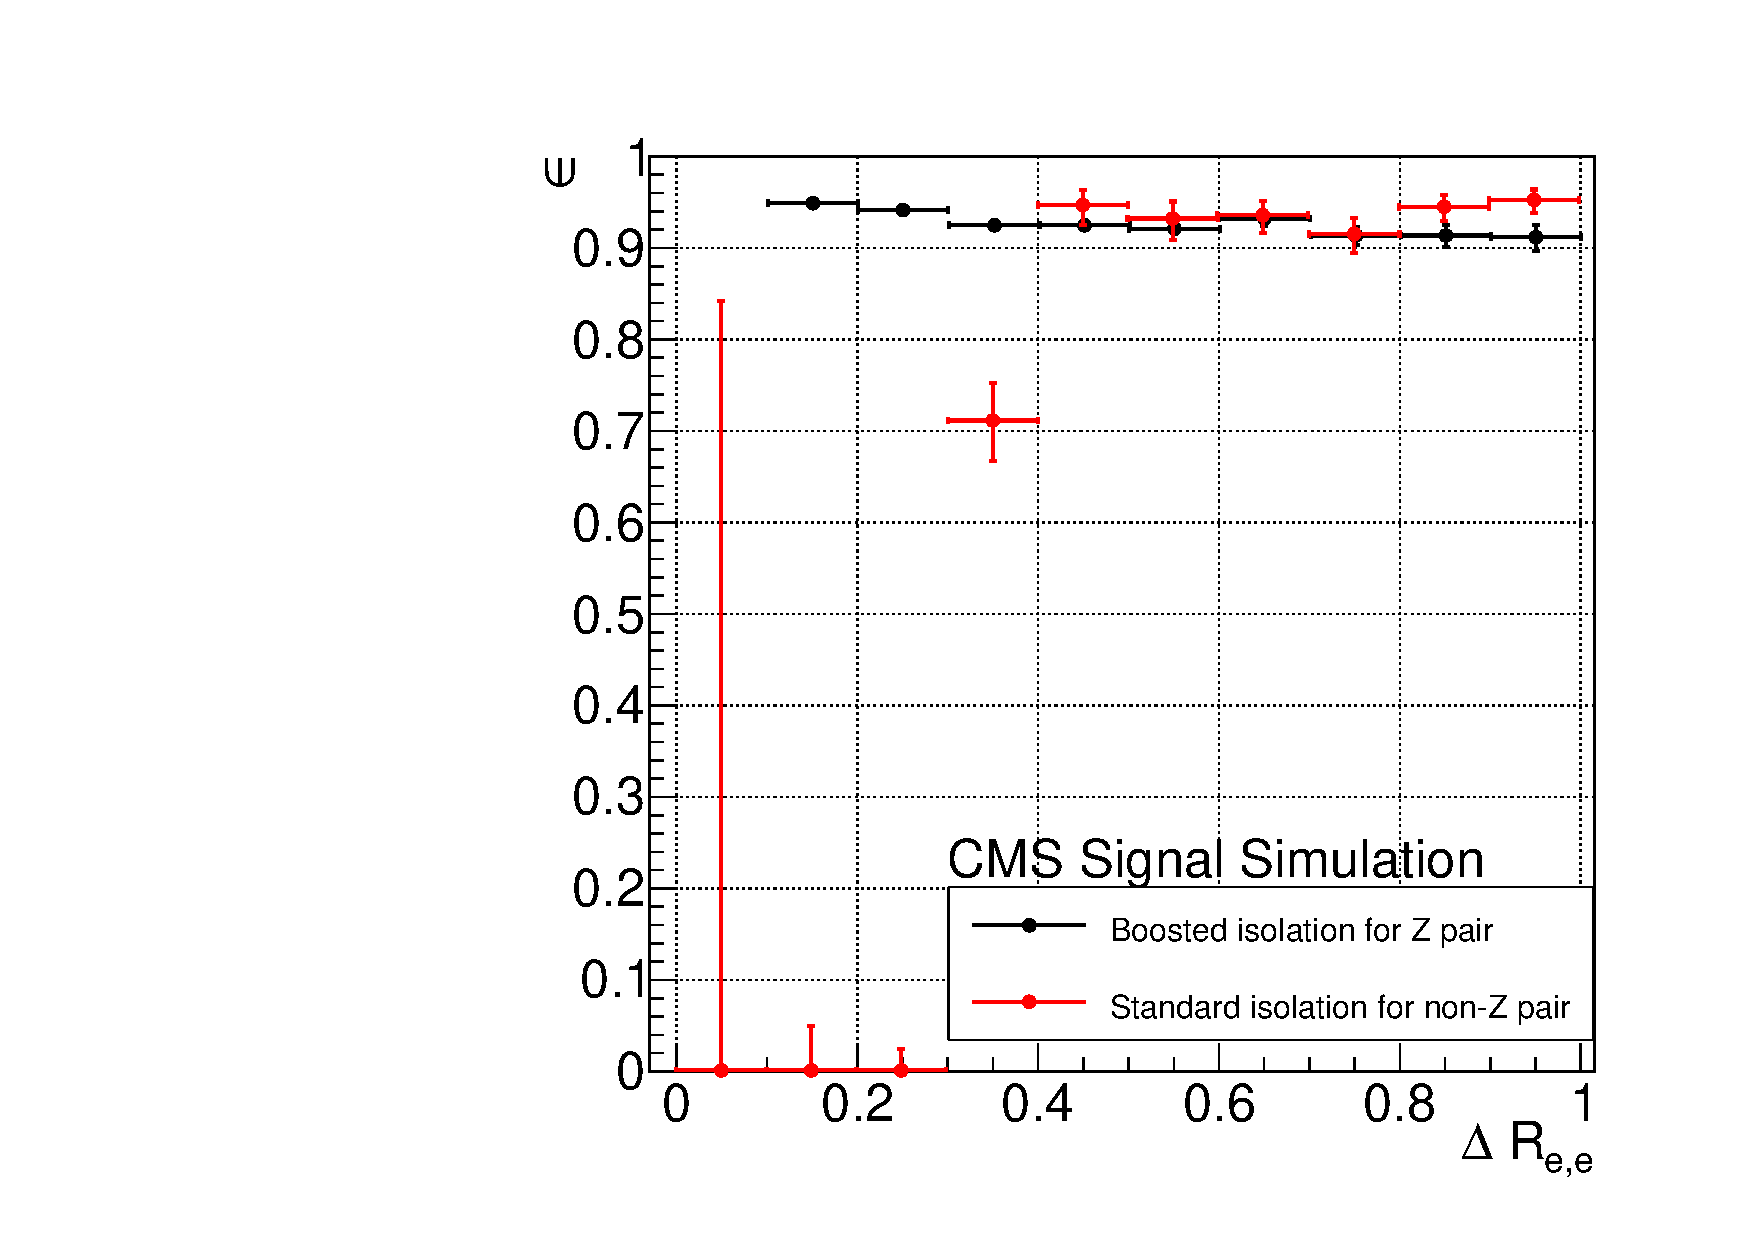
\includegraphics[width=0.5\textwidth]{plot/Isolation_muons.pdf}
\end{center} 
\caption{\label{fig:Iso_Eff}Efficiency of the isolation cut as a function of $\Delta R$ for electrons (top) and muons (bottom) for the non-Z pair with standard ID and the Z pair with boosted Z ID.}
\end{figure} 

%\begin{figure}[hp]
%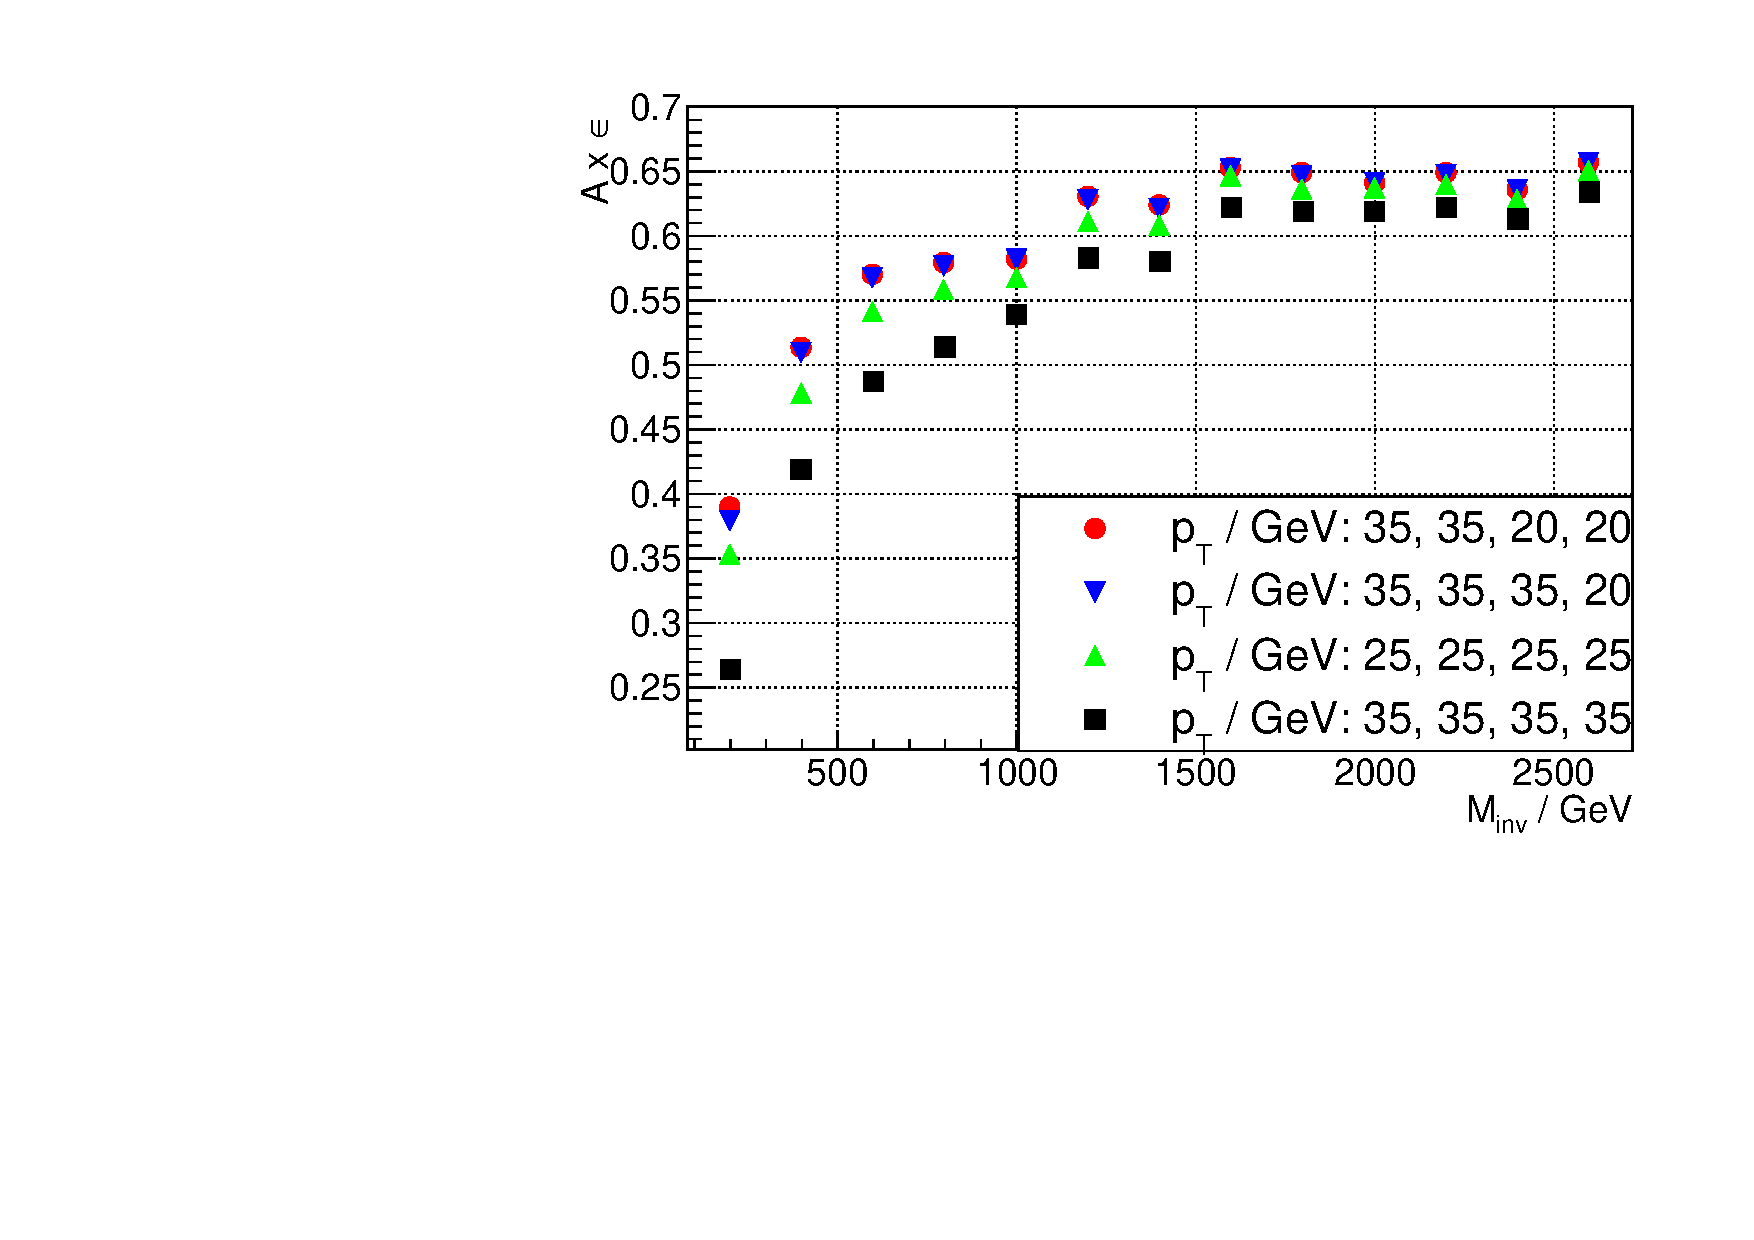
\includegraphics[width=\textwidth]{plots/AxE_Pt.pdf}
%\caption{Accpetance $\times$ efficiency for different $p_{T}$ for the 4$\mu$ channel. The later used acceptance cut of (25, 25, 25, 25) GeV has the same A $\times \epsilon$ as the green points (35, 35, 25, 25) GeV. For each signal, the two leading leptons have a $p_{T} >$ 35 GeV. }
%\end{figure}

\clearpage

\subsection{Pileup Reweighting}

The Monte Carlo samples are generated with a distribution for the number of pileup interactions in order to roughly match the conditions in data \cite{pileup}. However, there are differences between the pileup conditions in data and MC. Therefore, the pileup reweighting to MC samples is needed to account for the difference of pileup condition between data and MC. The Fig. \ref{fig:Vertices} shows the number of vertices after pileup reweighting. By applying a proper weight to each MC event according to data's pileup distribution, the MC samples can describes the data better.  

%\begin{figure}[hp]
%\begin{center}
%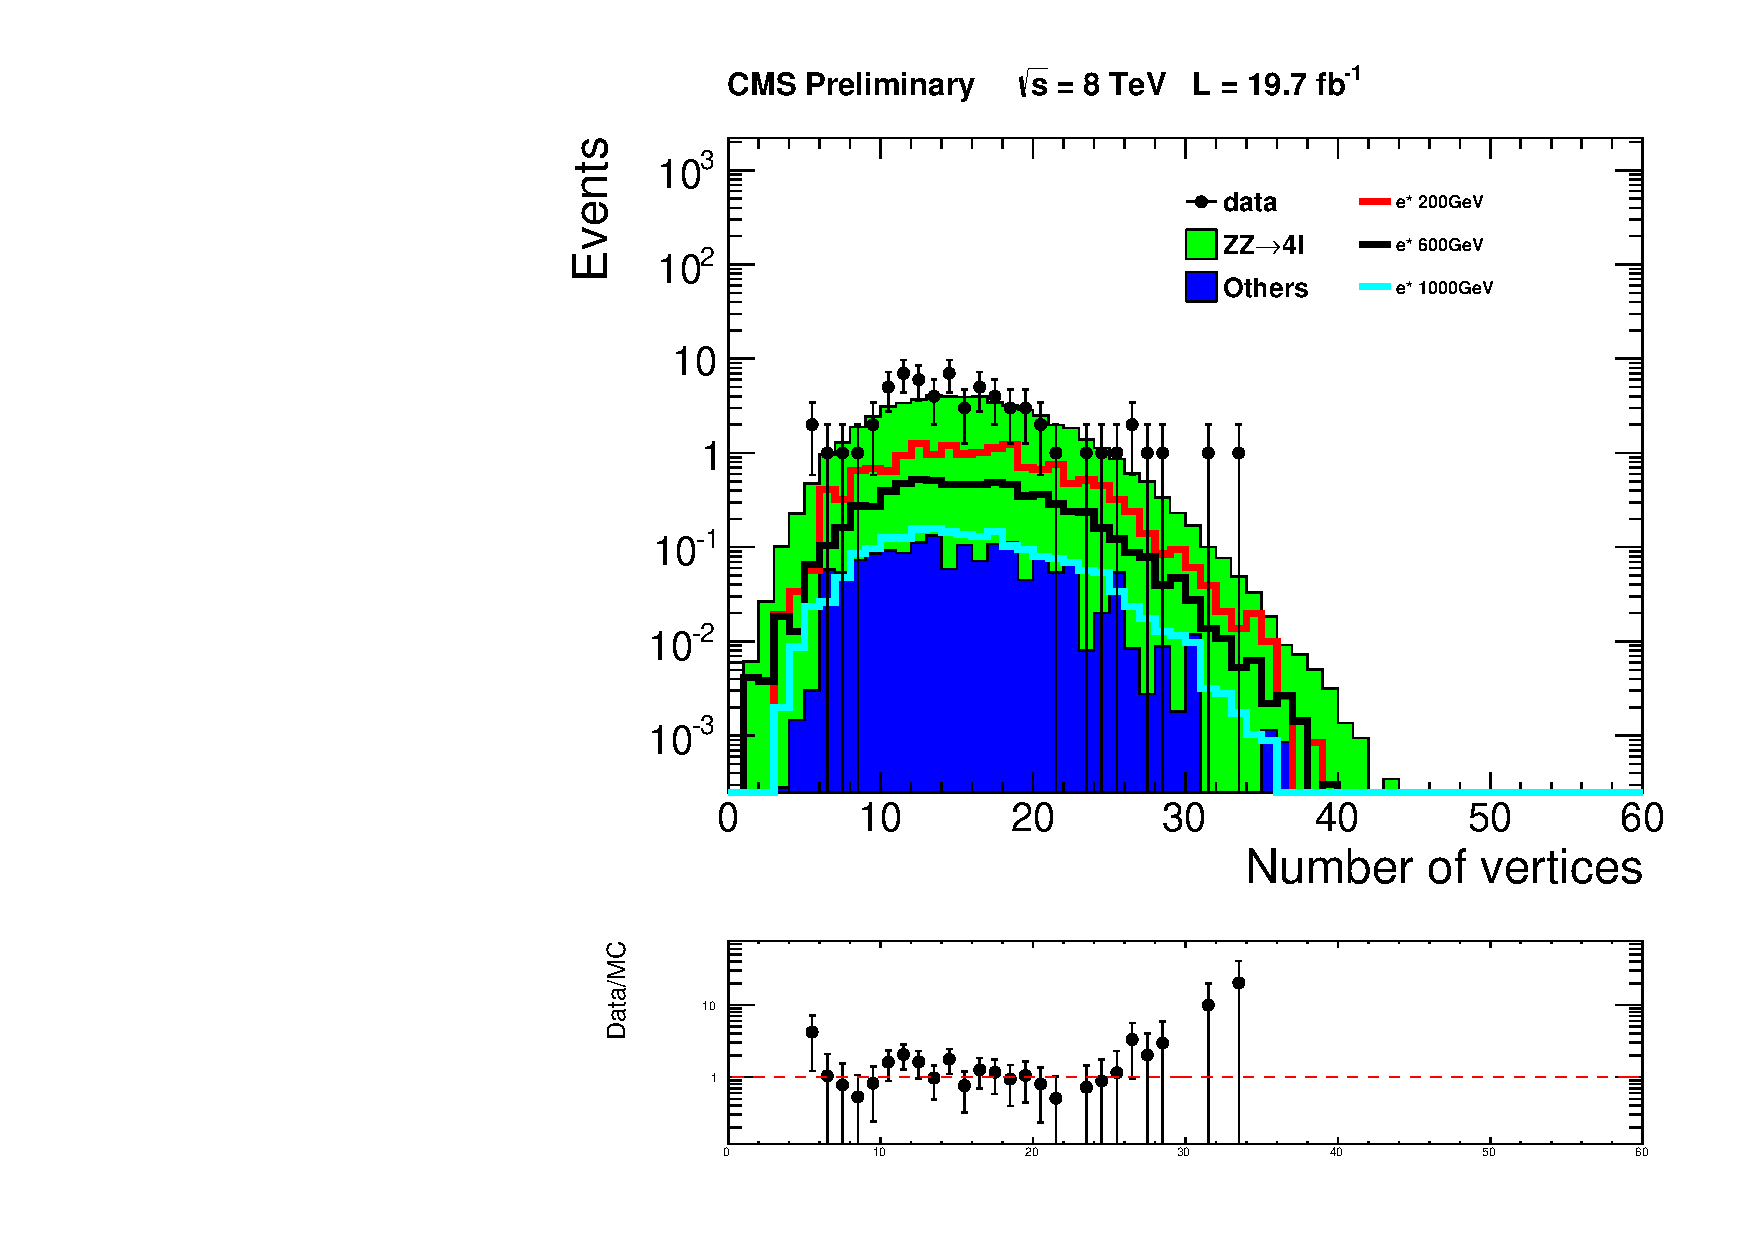
\includegraphics[width=0.48\textwidth]{plot/VtxN_2mu2e.pdf}
%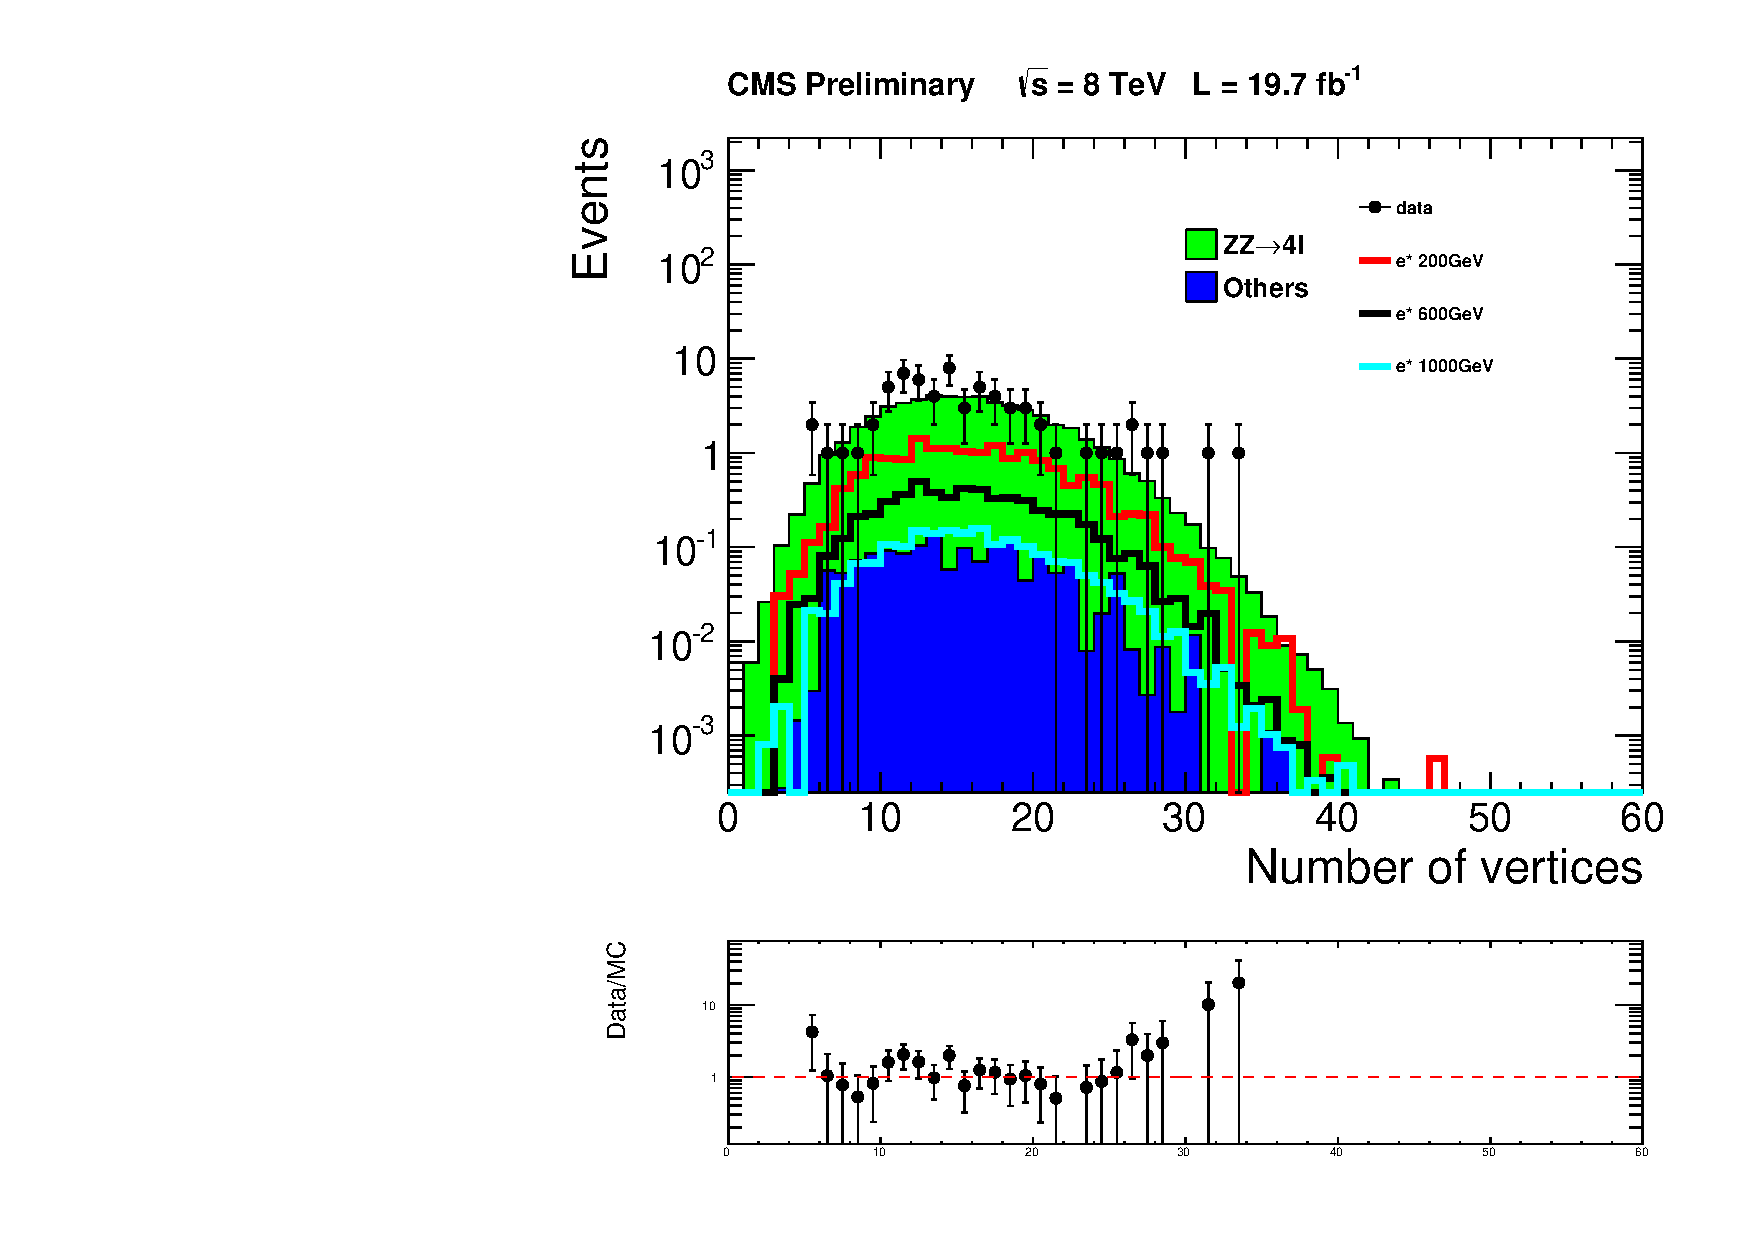
\includegraphics[width=0.48\textwidth]{plot/VtxN_2e2mu.pdf}
%\end{center} 
%\caption{\label{fig:Vertices_Bpu}Number of Vertices distribution before PileUp reweighting for $\mu\mu^{*} \rightarrow \mu\mu Z \rightarrow 2\mu2e$ (left), and $ee^{*} \rightarrow ee Z \rightarrow 2e2\mu$ (right).}
%\end{figure}  

\begin{figure}[hp]
\begin{center}
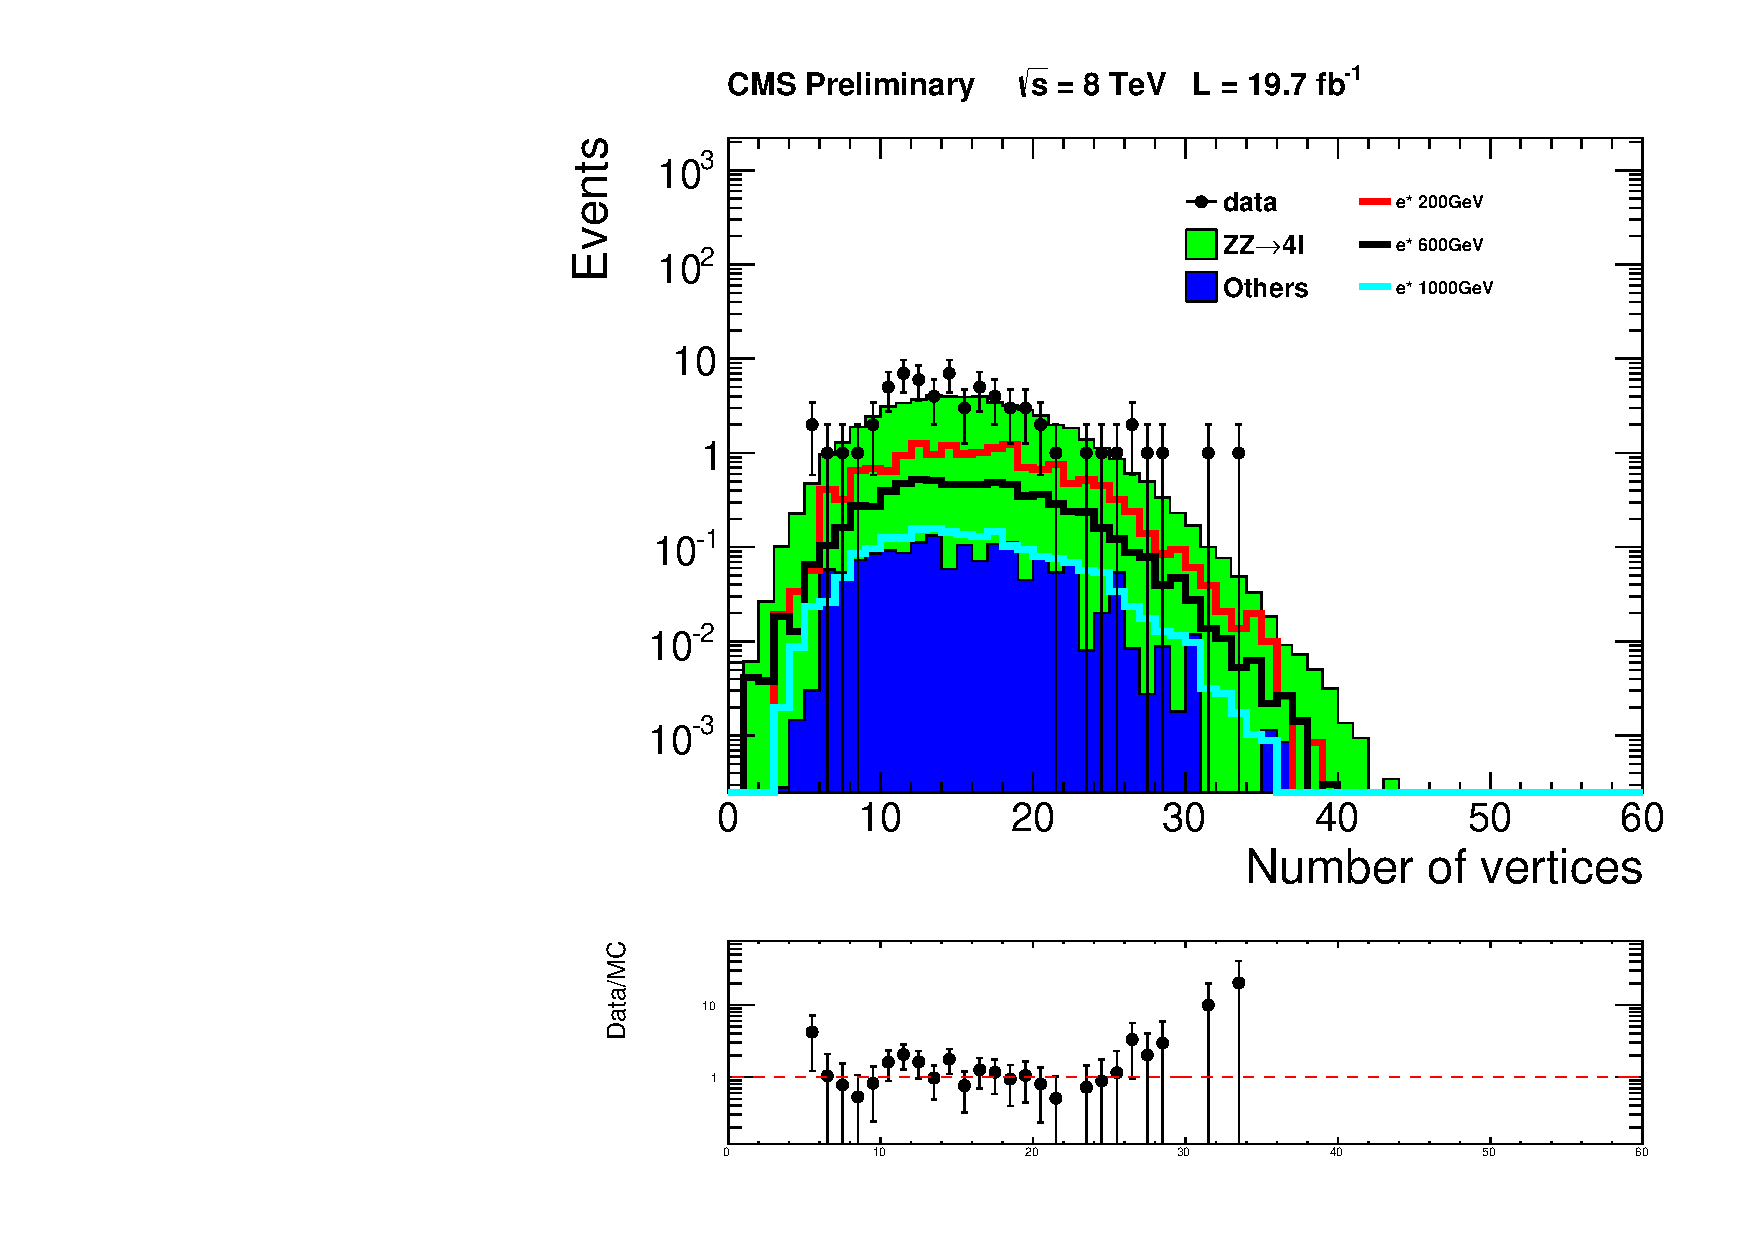
\includegraphics[width=0.48\textwidth]{plot/VtxN_2mu2e.pdf}
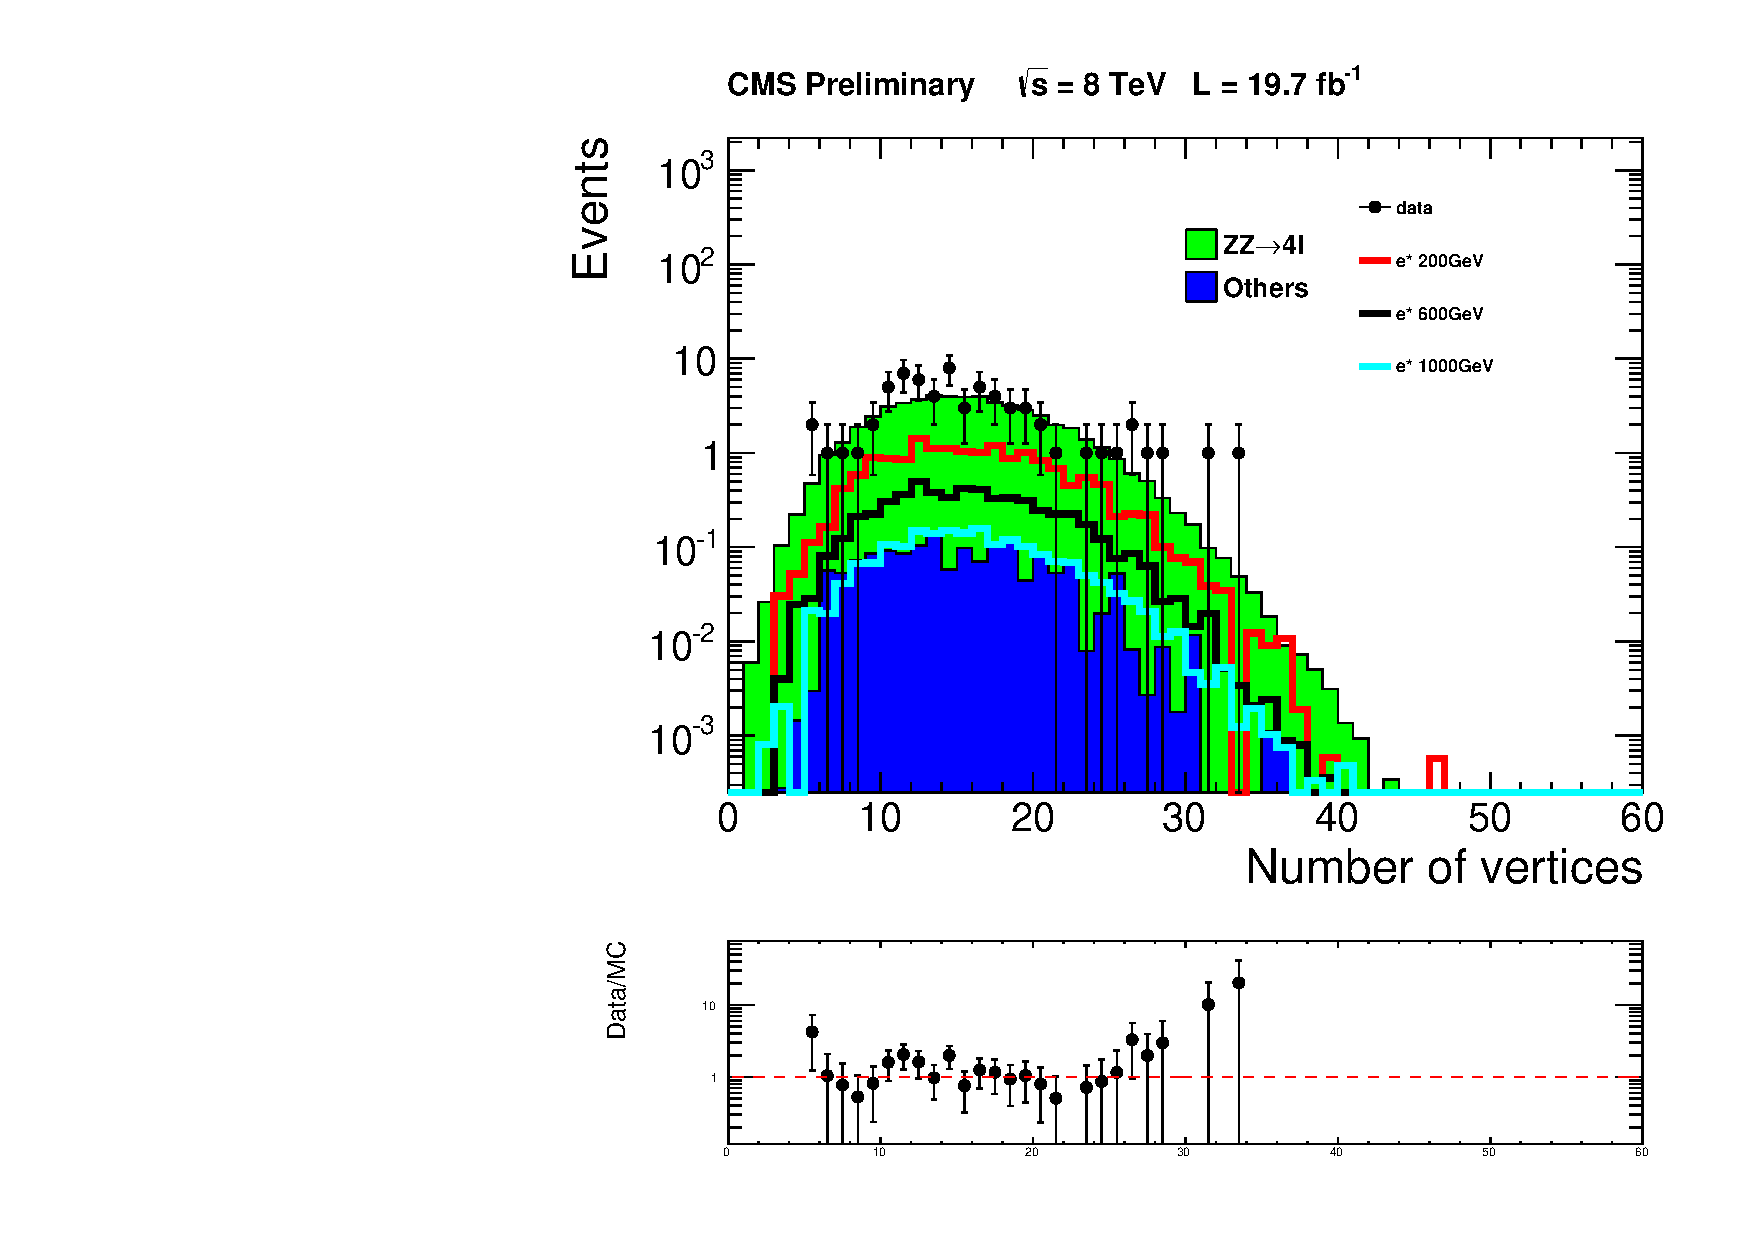
\includegraphics[width=0.48\textwidth]{plot/VtxN_2e2mu.pdf}
\end{center} 
\caption{\label{fig:Vertices}Number of Vertices distribution after PileUp reweighting for $\mu\mu^{*} \rightarrow \mu\mu Z \rightarrow 2\mu2e$ (left), and $ee^{*} \rightarrow ee Z \rightarrow 2e2\mu$ (right).}
\end{figure}  
